% This is "sig-alternate.tex" V2.0 May 2012
% This file should be compiled with V2.5 of "sig-alternate.cls" May 2012

\documentclass{sig-alternate}

\graphicspath{{./eps/}}
\DeclareGraphicsExtensions{.eps}

\usepackage{verbatim}
\usepackage{color}
\usepackage{subcaption}

\newdef{definition}{Definition}

\begin{document}

% --- Author Metadata here ---
%\conferenceinfo{WOODSTOCK}{'97 El Paso, Texas USA}
%\CopyrightYear{2007} % Allows default copyright year (20XX) to be over-ridden - IF NEED BE.
%\crdata{0-12345-67-8/90/01}  % Allows default copyright data (0-89791-88-6/97/05) to be over-ridden - IF NEED BE.
% --- End of Author Metadata ---

\title{Network Anomalies Detection}

\numberofauthors{3}

\author{
	\alignauthor
	Double Blind Submission
% The command \alignauthor (no curly braces needed) should
% precede each author name, affiliation/snail-mail address and
% e-mail address. Additionally, tag each line of
% affiliation/address with \affaddr, and tag the
% e-mail address with \email.
%
% 1st. author
% \alignauthor
% Ben Trovato\titlenote{Dr.~Trovato insisted his name be first.}\\
%        \affaddr{Institute for Clarity in Documentation}\\
%        \affaddr{1932 Wallamaloo Lane}\\
%        \affaddr{Wallamaloo, New Zealand}\\
%        \email{trovato@corporation.com}
% % 2nd. author
% \alignauthor
% G.K.M. Tobin\titlenote{The secretary disavows
% any knowledge of this author's actions.}\\
%        \affaddr{Institute for Clarity in Documentation}\\
%        \affaddr{P.O. Box 1212}\\
%        \affaddr{Dublin, Ohio 43017-6221}\\
%        \email{webmaster@marysville-ohio.com}
% % 3rd. author
}

\maketitle

\begin{abstract}
Abstract...
\end{abstract}

% A category with the (minimum) three required fields
%\category{H.2.8}{Database Applications}{Data Mining}
%A category including the fourth, optional field follows...
%\category{D.2.8}{Software Engineering}{Metrics}[complexity measures, performance measures]

%\terms{Theory}
%\terms{}
%\keywords{ACM proceedings, \LaTeX, text tagging}

\section{Introduction}
\label{sec:intro}
% The first paragraph of a research paper is always the hardest to write. Just write and ideas will flow while writing. (Writers' block)

In our increasingly complex world, networks offer an abstract representation for organizing the relationships between entities of interest in a complex system. The entities are represented as nodes while edges connecting pairs of nodes represent the existence of relationship between the entities. Examples of networks pervasive in our lives are social networks \cite{Wu2004}, protein networks, computer networks, transportation networks, neurological networks, organizational networks \cite{Mihm2010}, wireless sensor networks\footnote{Internet of Things}, electrical networks, etc. 

In these complex systems, a functional network that facilitates reliable flow of information through the edges is necessary for the complex system to achieve its objectives. However, it is inevitable that complex systems are subjected to wear and tear, leading to occasional anomalous behavior in certain parts of the system. Anomalies in the system would disrupt normal operations, and prevent the complex system from meeting its objectives.

While critical anomalies lead to catastrophic failures and cause the complete shutdown of a complex system, it is highly noticeable by the stakeholders of the complex system. The anomalies are thus quickly identified and localized for corrections to restore the functions of the complex system.

A more challenging \textbf{problem} which we address in our research, is to recognize the \emph{non-critical} anomalies that would result in a lower than optimal efficiency of the complex system. Such non-critical anomalies are often \emph{ignored} and its \emph{location unknown}, since the complex system can continue to function without corrections to them. But non-critical anomalies that are not corrected could aggravate over time into critical anomalies and cause catastrophic failure to the complex system in the unforeseeable future. 

Before proceeding further, we would use the Figures \ref{fig:travel_graph} and \ref{fig:7} to illustrate the problem. Figure \ref{fig:travel_graph} shows a small network where information flows from nodes to nodes through the directed edges. The edges connecting nodes $\{a, b, c, d, e\}$ form a path for information to flow between them. We do not assume that $a$ and $e$ is always the origin and destination of every information flow, i.e. users of the complex system could choose any of the intermediate nodes $\{b, c, d\}$ as origin or destination of their information journey. The \textcolor{red}{red $- ~ \cdot \rightarrow$} line indicates the possibility of an existing anomaly that would disrupt the flow of information along this route.

\begin{figure}[htb]
	\centering
	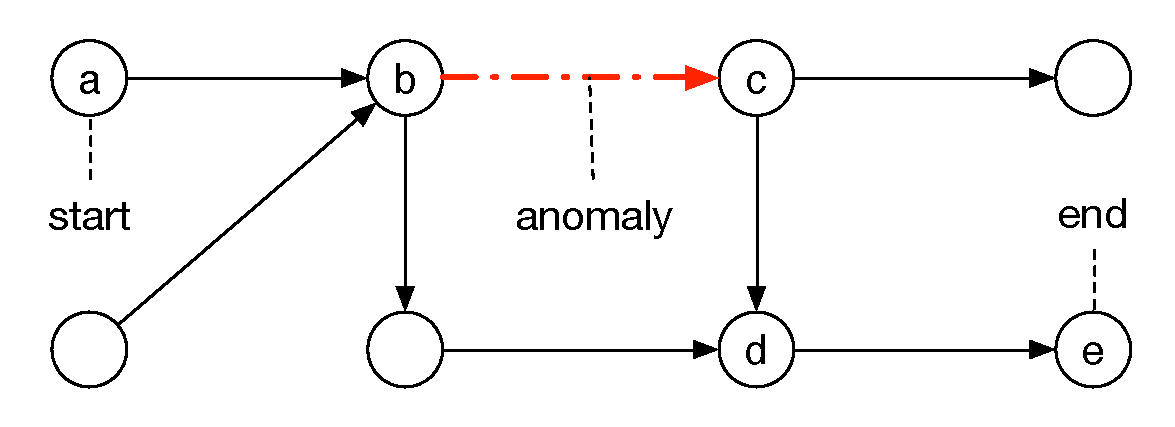
\includegraphics[width=3.3in]{travel_graph}
	\caption{Information Flow in Networks}
	\label{fig:travel_graph}
\end{figure}

Figures \ref{fig:7_start} and \ref{fig:7_end} show the histograms of information beginning its journey at the start node $a$, and ending its journey at the end node $e$. In the histograms, the x-axis represents the hour of the day, and each bin on the x-axis has a time interval of two minutes. The y-axis shows the number of journeys starting or ending its journey at the time corresponding to the timing of the bins. The phenomenon that we could immediately observe is that while the start node shows a \emph{regular} transmission of information, the end node receives the information at \emph{irregular} intervals. This could suggest the presence of an anomaly within the path such as the segment connecting node $b$ and $c$, suffering from a severe network congestion as shown in Figure \ref{fig:travel_graph}.

\begin{figure}[htb]
	\centering
	\begin{subfigure}{3.3in}
		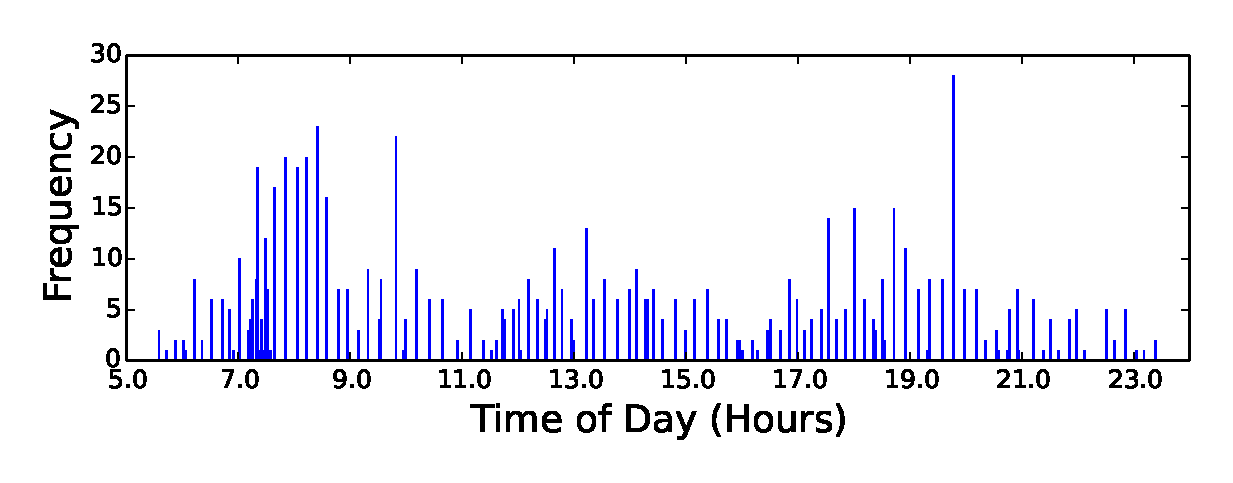
\includegraphics[width=3.3in]{7_start} %3.3in is max!
		\caption{Histogram at Start of Route}
		\label{fig:7_start}
	\end{subfigure}
	\begin{subfigure}{3.3in}
		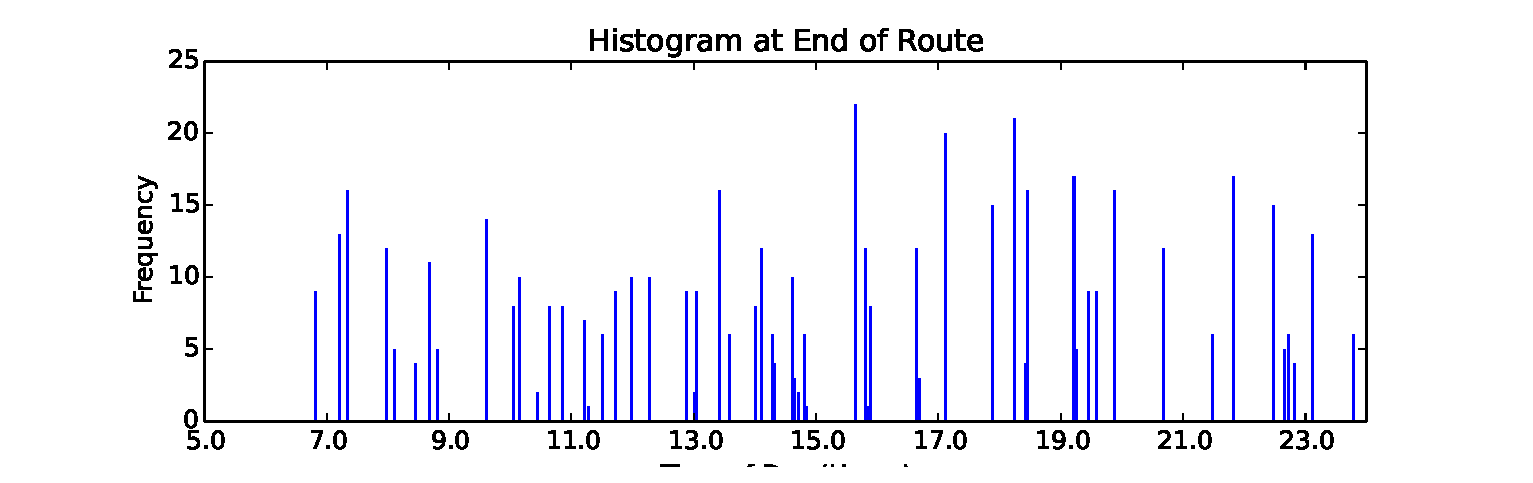
\includegraphics[width=3.3in]{7_end} %3.3in is max!
		\caption{Histogram at End of Route}
		\label{fig:7_end}
	\end{subfigure}
	\caption{Histograms of Information Flow}
	\label{fig:7}
\end{figure}

We propose a \emph{non-intrusive} solution to early detection of such anomalies in the rest of this paper. Our proposed non-intrusive \textbf{solution} relies on \emph{temporal} data related to the \emph{flow} of information from an \emph{origin} node to a \emph{destination} node. Since the solution should be non-intrusive, we only require temporal information from the two (origin and destination) end points while assuming that detailed temporal information during the journey is missing or difficult to obtain.

We formally define our problem based on the assumption that the following logged data is made available for our analysis. That is, given a set of records $R$ for a complex system, each record $r \in R$ contains the following,
\begin{enumerate}
	\item Spatial: The origin node $x_r$, and destination node $y_r$ of information flow in $r$.
	\item Temporal: The time $t(x_r)$ when information flow begins at the origin and the time $t(y_r)$ when information flow ends at the destination.
	\item Cost: The distance $d_r$ from $x_r$ to $y_r$ traveled by the information, or the non-temporal cost incurred due to the information flow.
	\item The path $p_r$ taken by $r$. The path consists of the sequence of nodes that the information visits for it to travel from node $x_r$ to node $y_r$. In situations where complete knowledge of the network or path is not known, it would still be possible to infer the path based on the distance traveled and intent of the information flow.
\end{enumerate}
A pair of consecutive nodes $i,j$ in path $p_r$, forms a segment $s_{i,j}$. We determine whether the time taken for information flow in $p_r$ deviates significantly from expectation. For all the records $r \in R$ with observed time that deviates significantly from the expected time, we locate the segments $s_{i,j} \in p_r$ that are likely to be the cause of the deviations.

This task is challenging due to the lack of data on the time it takes for information to flow through the individual segments. We need to infer the expected time for each segment based on the set of available records we have and the limited amount of data each record contains.

Our technical contribution is the proposal of a model that performs the inference on spatial-temporal data where knowledge of the temporal trajectory is missing or not available. Such situations are common when it is not possible to install sensors in complex systems for monitoring the temporal trajectory. For example, in computer networks, the application layer only have knowledge of the two endpoints while remaining oblivious to the intermediate nodes. Another example is transportation networks, which only records the passengers boarding and alighting stations for the purpose of calculating their transportation fare.

%The inference is only possible if the set of records are diverse in their origins and destinations. We would elaborate the proposed model in greater detail in Section \ref{sec:model}

\section{Related Work}
\label{sec:related}

\subsection{Traffic Anomalies Detection}

Pan et al. \cite{Pan2013} address the problem of detecting and describing traffic anomalies using crowd sensing with Beijing's taxis' GPS data and China's ``Weibo''\footnote{This service resembles Twitter but is catered for the Chinese population in Chinese language.} social media data. The anomaly which Pan et al. \cite{Pan2013} identifies is the deviance in traffic volume on segments of road during some special events. The detection of anomaly is relatively direct and the focus is on increasing the efficiency of the algorithm based on two special indexing structure for the detection algorithm.

Liu et al. \cite{Liu2011} proposed the discovery of causal interactions among traffic outliers. The framework as proposed in Liu et al.\cite{Liu2011} first partitions the geographical space into regions represented by nodes in a region graph. Edges between nodes represent the traffic flow between regions. Each edge in the region graph is differentiated within each time frame. By comparing the features of each edge across different time frames, Liu et al. is able to identify the outlier travel trajectories. From the detected outliers, an outlier tree is constructed with certain rules. In the outlier tree, each node represents an outlier trajectory. The parent of an outlier node occurs before in time and the destination of the parent is the origin of the child. The cause of the outlier, is the parent.

\cite{Ge2011,Zhang2011,Zhang2012} analyzed taxi GPS data to detect drivers who overcharge their passengers by deliberately taking the longer route to reach the destination. The general idea for finding these anomalous routes is to compare the route taken for each pickup and destination points and obtain a measure of how much it deviates from the usual routes.

Chawla et al. \cite{Chawla2012} proposed an algorithm to detect anomalies based Pinciple Component Analysis (PCA). Chawla et al. \cite{Chawla2012} represent the traffic data into two matrices, 1) the link-path matrix and the 2) link-time matrix. Then using PCA, Chawla et al. \cite{Chawla2012} is able to factorize the matrices into eigenvectors with its respective eigenvalues. The eigenvectors corresponding to large eigenvalues represent the norm, while those eigenvectors corresponding to lower eigenvalues represent the anomalies. Using these anomalies, Chawla et al. \cite{Chawla2012} tested their method to see if they could determine the root cause on synthetically generated data sets.

\section{Network Transmission Models}
\label{sec:models}

To find anomalies in the network, we analyse the set of information flow records $R$ from a complex system. But we must first determine which recorded information flow $r \in R$ is anomalous before we could proceed further with the localization task. A record $r$ is anomalous, if the observed time $\hat{t}_r$ taken to complete the distance $d_r$ deviates significantly from the expected value $t_r$ given to us by a statistical model.

\subsection{Baseline 1}

For our first baseline, we assume that every recorded information flow $r$ travels at a constant speed $c$ to cover the total distance $d_r$ required to reach its destination. The distribution of time taken $t_r$ for record $r$ is given by the following Gaussian distribution,
\[ t_r \sim \mathcal{N} \left( \frac{d_r}{c}, d_r \sigma^2 \right) \]
The unknown value of $c$ can be obtained by minimizing the following least squares error,
\[ \sum_{r \in R} (t_r - \hat{t}_r)^2 \]
Thus allowing us to obtain,
\begin{gather*}
	c = \frac{\sum_{r \in R} d_r}{\sum_{r \in R} \hat{t}_r} \qquad
    \sigma^2 = \frac{ \sum_{r \in R} \left( \hat{t}_r - \frac{d_r}{c} \right)^2 }{ \sum_{r \in R} d_r }
\end{gather*}

\subsection{Baseline 2}

The second baseline model which provides a more discriminative estimation than the first baseline is to assume a speed $c_p$ for each distinct path $p$ in the network.
\[ t_r \sim \mathcal{N} \left( \frac{d_r}{c_p}, d_r \sigma^2 \right) \]
The estimation for $c_p$ and $\sigma^2$ can be easily extended from the first baseline to obtain the following,
\begin{gather*}
	c_p = \frac{\sum_{r \in R_p} d_r}{\sum_{r \in R_p} \hat{t}_r} \qquad
    \sigma^2 = \frac{ \sum_{p \in P} \sum_{r \in R_p} \left( \hat{t}_r - \frac{d_r}{c_p} \right)^2 }{ \sum_{r \in R} d_r }
\end{gather*}
where $P$ is the set of possible paths and $R_p$ is the set of records that took the path $p \in P$.

\subsection{Edgebased Model}

We propose the Edgebased model, that models the speed of individual edges in the network. Given that an information flow record $r$ that originates from $x$ and terminates at $y$, the path taken by $r$ is denoted as $p_r$. Within each path $p_r$, the information flows through consecutive sequences of nodes. For every pair of consecutive node $i,j \in p_r$, the segment $s_{i,j}$ connecting the pair is associated with the known distance $d_{i,j}$ and an estimated speed $c_{i,j}$. The time taken $t_{i,j}$ for each segment $s_{i,j}$ could then be estimated using the distance $d_{i,j}$ and speed $c_{i,j}$. Summation of the estimated time in each segment gives the expected time $t_r$ needed for $r$ to travel from $x$ to $y$.

The distribution of time for each segment $s_{i,j}$ is given by the following Gaussian distribution,
\[ t_{i,j} \sim \mathcal{N} \left( \frac{d_{i,j}}{c_{i,j}}, d_{i,j} \sigma^2 \right) \]

The distribution of time $t_r$ of $r$ is given by the following linear Gaussian distribution,
\begin{align*}
	t_r &= \sum_{ (i,j) \in p_r } t_{i,j} \\
	t_r &\sim \mathcal{N} \left( \sum_{ (i,j) \in p_r } \frac{ d_{i,j} }{ c_{i,j} }, d_r \sigma^2 \right)
\end{align*}
To estimate the variance $\sigma^2$,
\begin{align*}
	\sigma^2 = \frac{ \sum_{r \in R} \left( \hat{t}_r - \sum_{ (i,j) \in p_r } \frac{d_{i,j}}{c_{i,j}} \right)^2}{\sum_{r \in R} d_r}
\end{align*}

To estimate the speed $c_{i,j}$ of every segment $s_{i,j}$ using the observed time $\hat{t}_r$ of each record $r$, we maximize the log likelihood from each $r$. The log likelihood as contributed by $r$ is given by,
\begin{align*}
	\mathcal{L}_r &= \log \left( \frac{1}{\sqrt{2 \pi d_r \sigma^2 }} \right) - \frac{\left( \hat{t}_r - \sum_{ (i,j) \in p_r } \frac{d_{i,j}}{c_{i,j}} \right)^2}{2 d_r \sigma^2 } \\
	&= - \frac{1}{2} \log \left( d_r \sigma^2 \right) - \frac{\left( \hat{t}_r - \sum_{ (i,j) \in p_r } \frac{d_{i,j}}{c_{i,j}} \right)^2}{2 d_r \sigma^2 }
\end{align*}
We add a log barrier penalty to prevent negative speeds,
\begin{align}
	\label{eqn:objective1}
	\mathcal{L}^*_r = \mathcal{L}_r + \tau \sum_{(i,j) \in p_r} \log c_{i,j}
\end{align}
By taking partial derivative with respect to $c_{p,q}$,
\begin{align}
	\label{eqn:sgd_mean}
	\frac{\partial \mathcal{L}^*_r}{\partial c_{p,q}} = - \frac{\left( \hat{t}_r - \sum_{ (i,j) \in p_r } \frac{d_{i,j}}{c_{i,j}} \right)}{d_r \sigma^2 } \cdot \frac{d_{p,q}}{c_{p,q}^2} + \frac{\tau}{c_{p,q}}
\end{align}
The partial derivative allows us to perform Stochastic Gradient Descent (SGD) on parameters $c_{i,j}$ as follows,
\begin{align*}
	%\label{eqn:update}
	c_{i,j} \leftarrow c_{i,j} + \eta \frac{\partial \mathcal{L}^*_r}{\partial c_{i,j}}
\end{align*}
There are several interesting properties with the partial derivative in Equation \ref{eqn:sgd_mean}. The variance in the denominator shows that the more uncertain we are, the lesser the gradient is, hence less changes to $c_{i,j}$. The smaller $c_{i,j}$ is, the second component in Equation \ref{eqn:sgd_mean} will compensate by adding positive value to prevent $c_{i,j}$ from entering the negative region.

\subsection{Smoothed Edgebased Model}

To avoid overfitting the model parameters to the observed data set, we add additional constraints to Equation \ref{eqn:objective1} that minimize the difference between the speeds of consecutive segments in a path. This constraint is based on the assumption that consecutive segments have related speeds.
\begin{align*}
	\mathcal{L}^{**}_r = \mathcal{L}^*_r - \frac{\psi}{2} \sum_{(i,j) \in p_r} \left( c_{i,j} - c_{j,k} \right)^2
\end{align*}
where $c_{j,k}$ is speed of $s_{j,k}$ that comes after $s_{i,j}$.

Estimation for the variance $\sigma^2$ remains the same while estimation of $c_{i,j}$ is slightly modified,
\begin{align*}
	\frac{\partial \mathcal{L}^{**}_r}{\partial c_{i,j}} &= \frac{\partial \mathcal{L}^*_r}{\partial c_{i,j}} - \psi (c_{i,j} - c_{j,k}) \\
	c_{i,j} &\leftarrow c_{i,j} + \eta \frac{\partial \mathcal{L}^{**}_r}{\partial c_{i,j}}
\end{align*}

In Section \ref{sec:experiments}, we would evaluate which of these models is a better choice in terms of generalizing to records that are not observed during the estimation (training) phase.

\section{Localization of Network Anomalies}
\label{sec:localization}

The models as described in previous section would allow us to determine whether a record $r \in R$ is anomalous by comparing the difference of the observed time and the expected time $\hat{t}_r - t_r$ with the standard deviation $\sqrt{d_r \sigma^2}$. We use the following ratio $\alpha_r$ to measure the degree of deviation.
\begin{align*}
	%\label{eqn:alpha_ratio}
	\alpha_r = \frac{\hat{t}_r - t_r}{\sigma \sqrt{d_r}}
\end{align*}

For records $r \in R$ with $\alpha_r > 1$, it indicates that the time taken is longer than expected while $\alpha_r < 1$ indicates that the time taken is shorter than expected. In most complex systems, the records of interest for further investigation would be records with $\alpha_r > \delta$, where $\delta$ is a cut-off value to determine whether $r$ has a larger observed time than expected. We would be able to obtain a reduced set of records $R_{\alpha > \delta}$ such that $r \in R_{\alpha > \delta}$ has a ratio $\alpha_r > \delta$ for further investigation.

But a high ratio $\alpha_r$ for record $r \in R_{\alpha > \delta}$ could be an isolated incident that does not have any significant impact on the complex system. The ratio $\alpha_r$ also does not reveal the specific segment $s_{i,j}$ in the path $p_r$ of $r$ that causes the longer observed time $\hat{t}_r$. To address these issues, we propose an algorithm that serve two purposes:
\begin{enumerate}
	\item Measuring how many other records $r' \in R_{\alpha > \delta}\setminus{r}$ are related to $r$ in order to determine the significance of the network congestion in the path $p_r$ taken by $r$.
	\item Locating the segment $s_{i,j} \in p_r$ that is most likely to contribute to the high $\alpha_r$ ratio of $r$.
\end{enumerate}
We first define the ``relatedness'' of two records $r, r'$ in more precise terms using ``contains'' and ``within''.
\begin{definition}
	$r'$ contains $r$ if all of the following conditions are satisfied: 
	\begin{enumerate}
		\item The path $p_{r'}$ connecting the origin $x_{r'}$ and destination $y_{r'}$ of $r'$, passes through the path $p_{r}$ that connects the origin $x_{r}$ and destination $y_{r}$ of $r$. 
		\item The time $t(x_{r'})$ when $r'$ starts at origin $x_{r'}$, is earlier than the time $t(x_{r})$ when $r$ starts at origin $x_{r}$. i.e. $t(x_{r'}) < t(x_{r})$.
		\item The time $t(y_{r'})$ when $r'$ ends at destination $y_{r'}$, is later than the time $t(x_{r})$ when $r$ ends at destination $y_{r}$. i.e. $t(y_{r'}) > t(y_{r})$.
	\end{enumerate}
\end{definition}
\begin{definition}
	$r$ is within $r'$ if and only if $r'$ contains $r$.
\end{definition}
Based on the two definitions, the algorithm for localizing the anomalies in the network proceed as follows:
\begin{enumerate}
	\item Obtain the set of records $R_{\alpha > \delta}$ such that $r \in R_{\alpha > \delta}$ has a ratio $\alpha_r > \delta$.
	\item For each $r \in R_{\alpha > \delta}$, obtain the set of records $R_r$,
	\[ R_{r} := \{ r' \in R_{\alpha > \delta} | r' ~ \text{contains} ~ r \land r' \neq r \} \]
	%such that each $r' \in R_r$ contains $r$, $r' \neq r$ and $$.
	\item Then by sorting $r \in R_{\alpha > \delta}$ in descending order of $|R_r|$, and examining the segments $s_{i,j}$ of path $p_r$, we would be able to locate the segments $s_{i,j}$ with severe network congestion between the times of $t(x_r)$ and $t(y_r)$.
	\item For any given $r' \in R_{\alpha > \delta}$, we would also be able to locate the congested segments of path $p_{r'}$ by using the path $p_r$ of records $r$, where $r$ is within $r'$ and $R_r = \emptyset$.
\end{enumerate}

\section{Experiments}
\label{sec:experiments}

We first apply the models from Section \ref{sec:models} on the data set of a complex system to test the generalization performance. The model that has the best generalization performance would have the lowest prediction error for unobserved data. We then select the best model to use for detection and localization of network anomalies in the complex system by applying the algorithm as described in Section \ref{sec:localization}. To evaluate on the reliability of the detected and localized anomalies, we examine the Twitter records of the same period to check whether users of the complex system expressed their frustrations by tweeting (complaining) on Twitter.

\subsection{Data Description}

We test our models on a data set that contains the passengers' travel records on the Public Transportation System (PTS) of Singapore\footnote{http://en.wikipedia.org/wiki/Singapore}, a highly urbanized sovereign city-state located in Southeast Asia. The PTS consists of the railway system\footnote{http://en.wikipedia.org/wiki/SMRT\_Corporation} and the public buses\footnote{http://en.wikipedia.org/wiki/SBS\_Transit}, operated by two public listed corporations. The PTS data set is provided by the city's transportation authority\footnote{http://en.wikipedia.org/wiki/Land\_Transport\_Authority} that monitors the transportation needs of the city for her economic activities.

Each passenger in Singapore carries a payment card containing a RFID chip. The RFID chip allows the companies to identify the passenger and charge the transportation fare to their account. The passengers boarding and alighting geo-locations are recorded for each travel trip in order to charge the appropriate amount based on the distance traveled. The time boarded and time alighted are also recorded, which makes it possible to calculate the time taken for the travel.

Singapore being one of the most densely populated city in the world, have majority of her population commuting via the PTS, as opposed to driving in privately owned vehicles. The data set thus represent an almost complete usage of a real and large-scale complex system, which would allow us to utilize it for verifying our proposed models and algorithms.

We mentioned in Section \ref{sec:intro} that we wanted to detect non-critical anomalies because it is less noticeable than critical anomalies. The transportation network of bus routes would contain many of these non-critical anomalies because traffic in congested road segments can be diverted to other roads. On the other hand, anomalies in the railway system are easily detected because trains in the same direction travel on a single railway track. For the purpose of verifying our models and algorithms, we only focus on the bus records for the rest of this paper. Each record $r$ contains the following information of a passenger's journey:
\begin{enumerate}
	\item Bus stop ID of boarding, $x_r$.
	\item Bus stop ID of alighting, $y_r$.
	\item Date and time of boarding, $t(x_r)$.
	\item Date and time of alighting, $t(y_r)$.
	\item Distance traveled between boarding and alighting, $d_r$.
	\item Bus service: The bus service is a number, which represents the unique route taken by the bus. Many different buses operate using the same service number so that different buses can pick up or alight passengers at various bus stops with regular intervals. Using the bus service number, the bus stop ID of boarding and alighting, we are able to obtain the path $p_r$ traveled by the passenger of this record $r$.
\end{enumerate}
The bus routes remain relatively static but may change due to road maintenance and repairs. To ensure that we always have the correct bus routes for each specific bus service, we perform a simple bus route inference step in the next section.

\subsubsection{Bus Route Inference}

Figure \ref{fig:trip_example} shows an example of three records for the \emph{same} bus service number. We have the time and location of the passenger boarding and alighting from the bus for each of their journeys. The nodes in Figure \ref{fig:trip_example} represent the bus stops while the number in the connecting edges represent the distance between two bus stops. By using different records of the same bus service, we are able to construct the route that the bus service takes, as shown in Figure \ref{fig:trip_example}. For example, from Figure \ref{fig:trip_example}, we can infer that $b$ should be between $a$ and $c$ because $b$ is nearer to $c$ compared to $a$, and $c$ is nearer to $b$ than $d$ so $d$ should come after $c$.
\begin{figure}[htb]
	\centering
	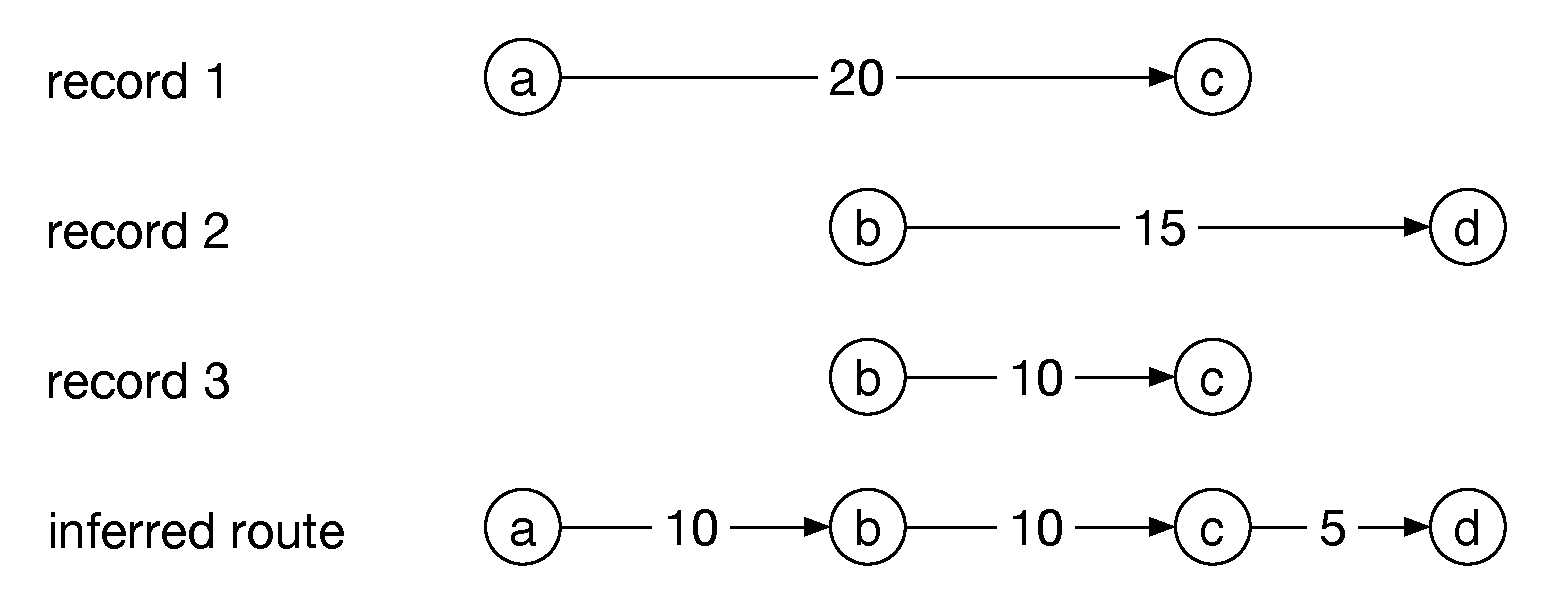
\includegraphics[width=3.3in]{trip_example}
	\caption{Examples of the trip records in the data set for a specific bus service}
	\label{fig:trip_example}
\end{figure}
Then by combining the inferred routes of various bus services, we would be able to obtain a transportation network as shown in Figure \ref{fig:travel_graph} of Section \ref{sec:intro}. %Using the time information in the data set, our proposed models in Section \ref{sec:models} and the localization algorithm in Section \ref{sec:localization}, we would be able to obtain the edges in red, which represent the roads that contain anomalies, resulting in the longer than expected timings of bus arrivals at bus stops. %Because of the time information in the data set, we would have a continuous snapshot of the traffic graph at different times.

\subsubsection{Statistics}

We performed our analysis on three days of data, December 8th 2011, December 15th 2011 and December 22nd 2011. These three days are spaced one week apart and falls on Thursday of the week, which is a typical working day. The reason for choosing these specific days is because of the occurrence of an event (external to the bus system) on December 15th 2011 which affected the transportation system of the city. The choice of December 8th and December 22nd is to show that the anomalies present on December 15th, is absent one week before and one week after. 

\begin{table}[htb]
	\centering
	\caption{Size of data set for each day}
	\label{tbl:statistics}
	\begin{tabular}{|p{1in}|r|r|r|}
		\hline
			& Dec 8th & Dec 15th & Dec 22nd \\
		\hline
		No. of records & 3,137,469 & 3,176,830 & 3,162,985\\
		\hline
		No. of inferred bus routes & 288 & 285 & 287\\
		\hline
		No. of nodes & & &\\
		\hline
		No. of edges & & &\\
		\hline
	\end{tabular}
\end{table}



\subsection{Sum-of-Squares Error Convergence}
Figure \ref{fig:convergence}.
\begin{figure}[htb]
	\centering
	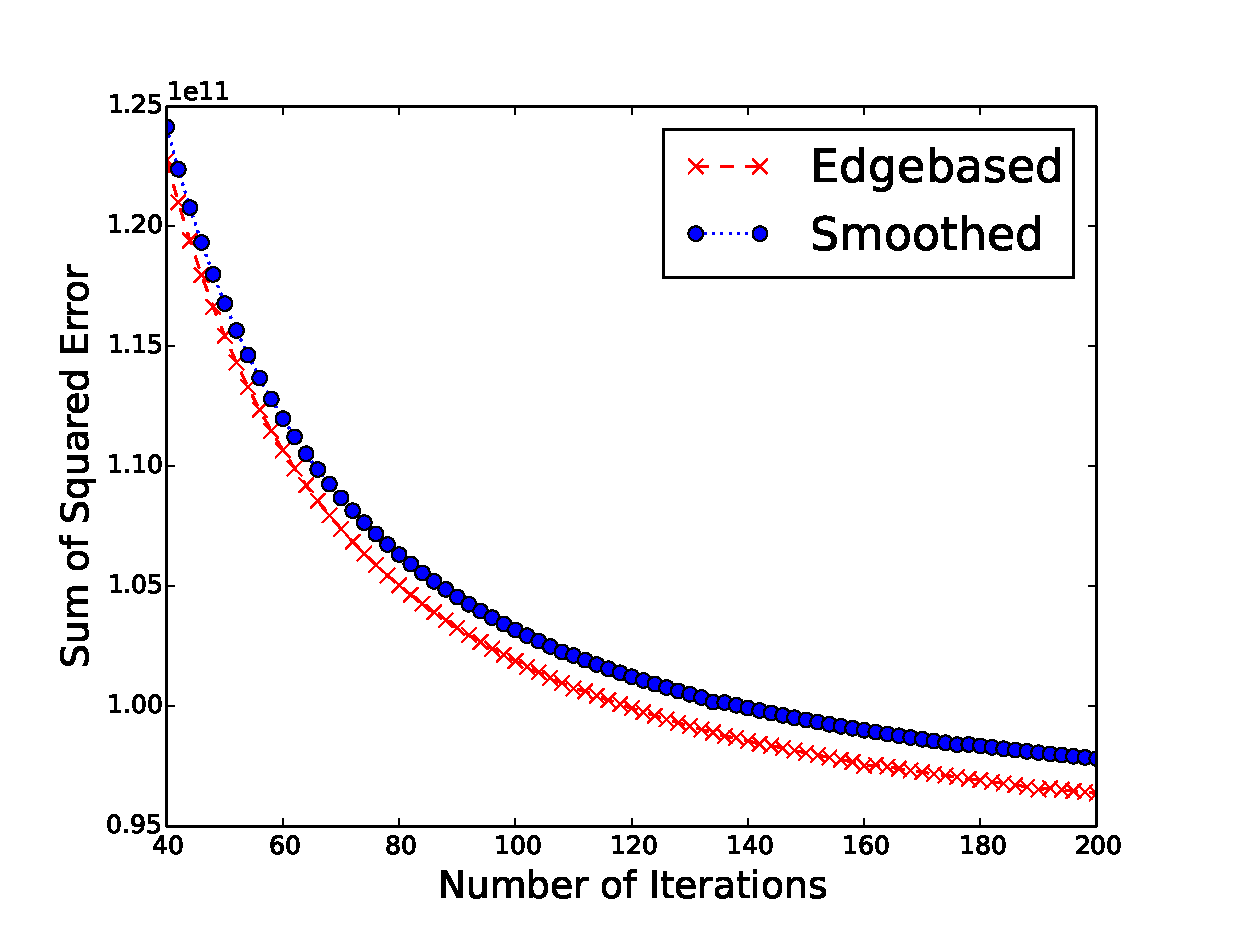
\includegraphics[width=3.3in]{convergence}
	\caption{Stochastic Gradient Descent Convergence rate for Sum of Squared Error}
	\label{fig:convergence}
\end{figure}

\subsection{K-Fold Cross Validation}
Figure \ref{fig:5_fold_train} and \ref{fig:5_fold_test}.
\begin{figure}[htb]
	\centering
	\begin{subfigure}{1.6in}
		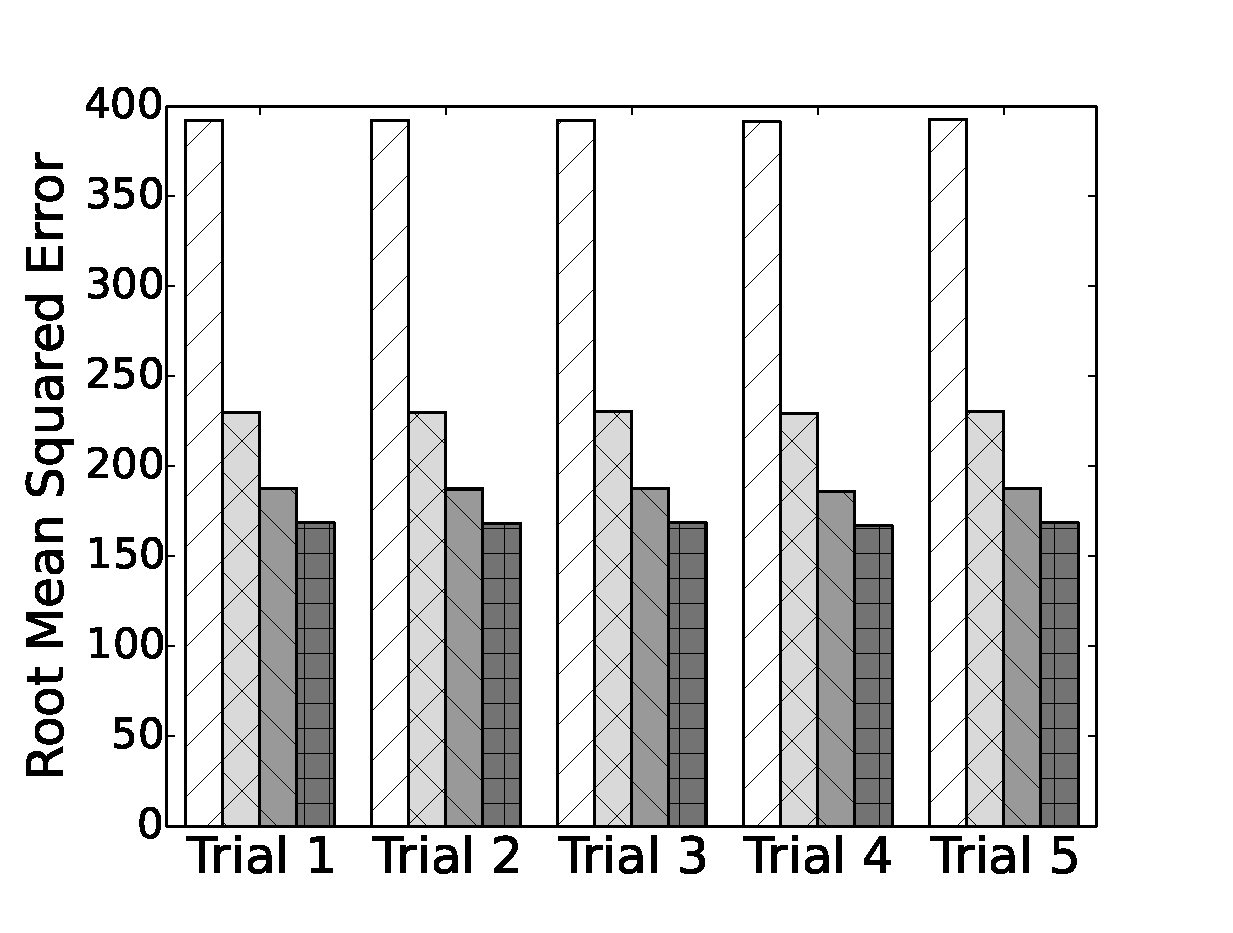
\includegraphics[width=1.6in]{20111208_train} %3.3in is max!
		\caption{Dec 8th 2011}
		\label{fig:20111208_train}
	\end{subfigure}
	\begin{subfigure}{1.6in}
		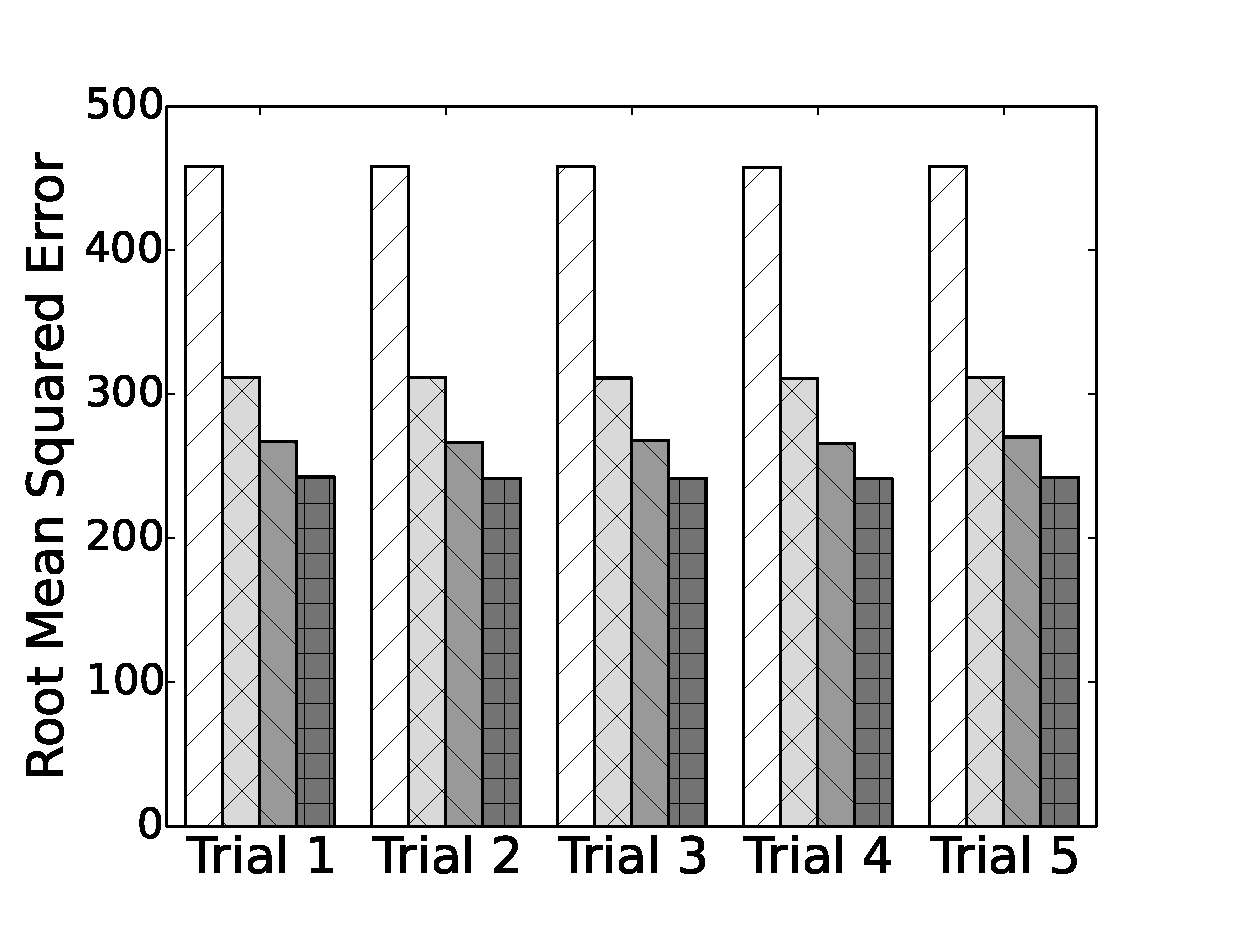
\includegraphics[width=1.6in]{20111215_train} %3.3in is max!
		\caption{Dec 15th 2011}
		\label{fig:20111215_train}
	\end{subfigure}
	\begin{subfigure}{1.6in}
		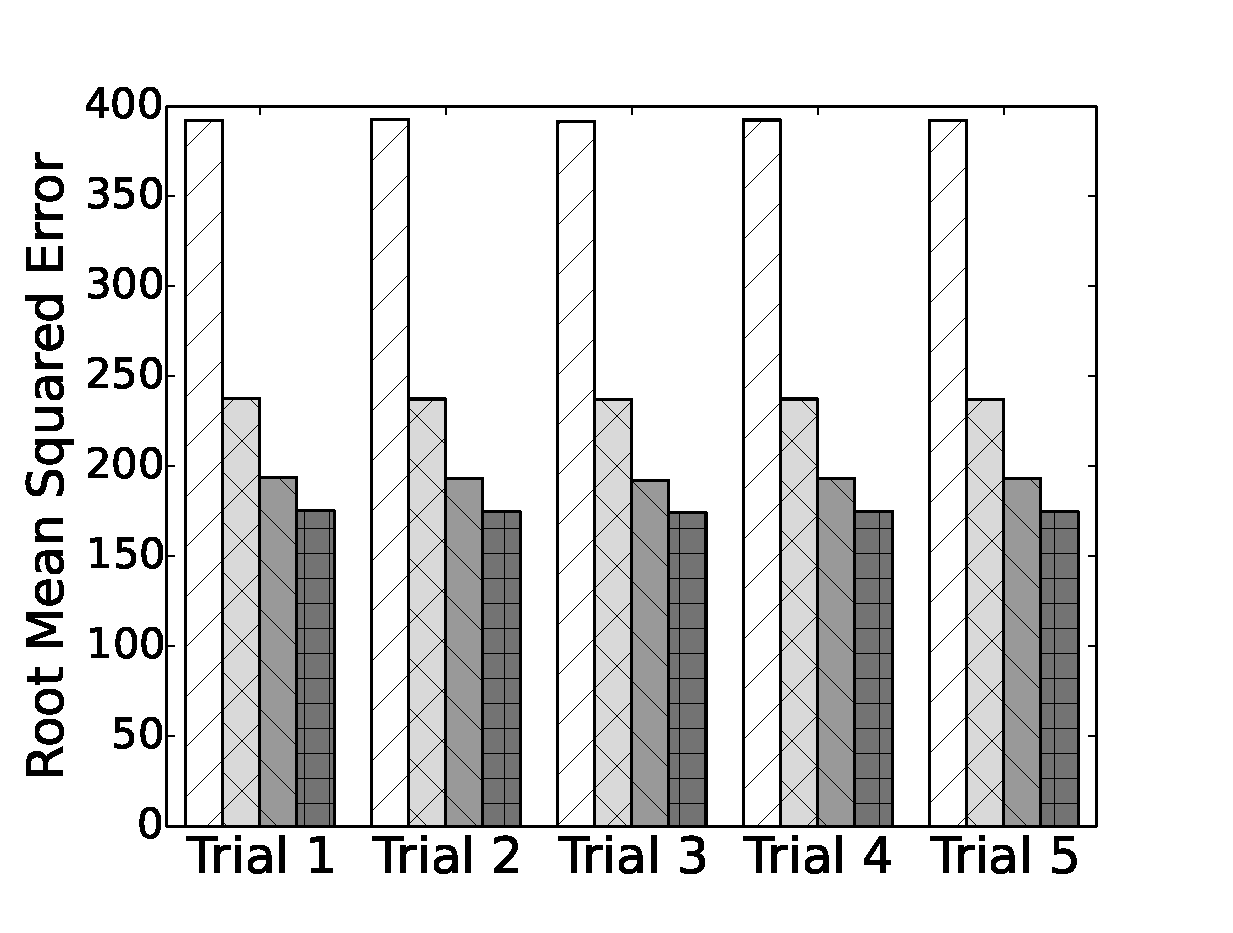
\includegraphics[width=1.6in]{20111222_train} %3.3in is max!
		\caption{Dec 22nd 2011}
		\label{fig:20111222_train}
	\end{subfigure}
	\begin{subfigure}{1.6in}
		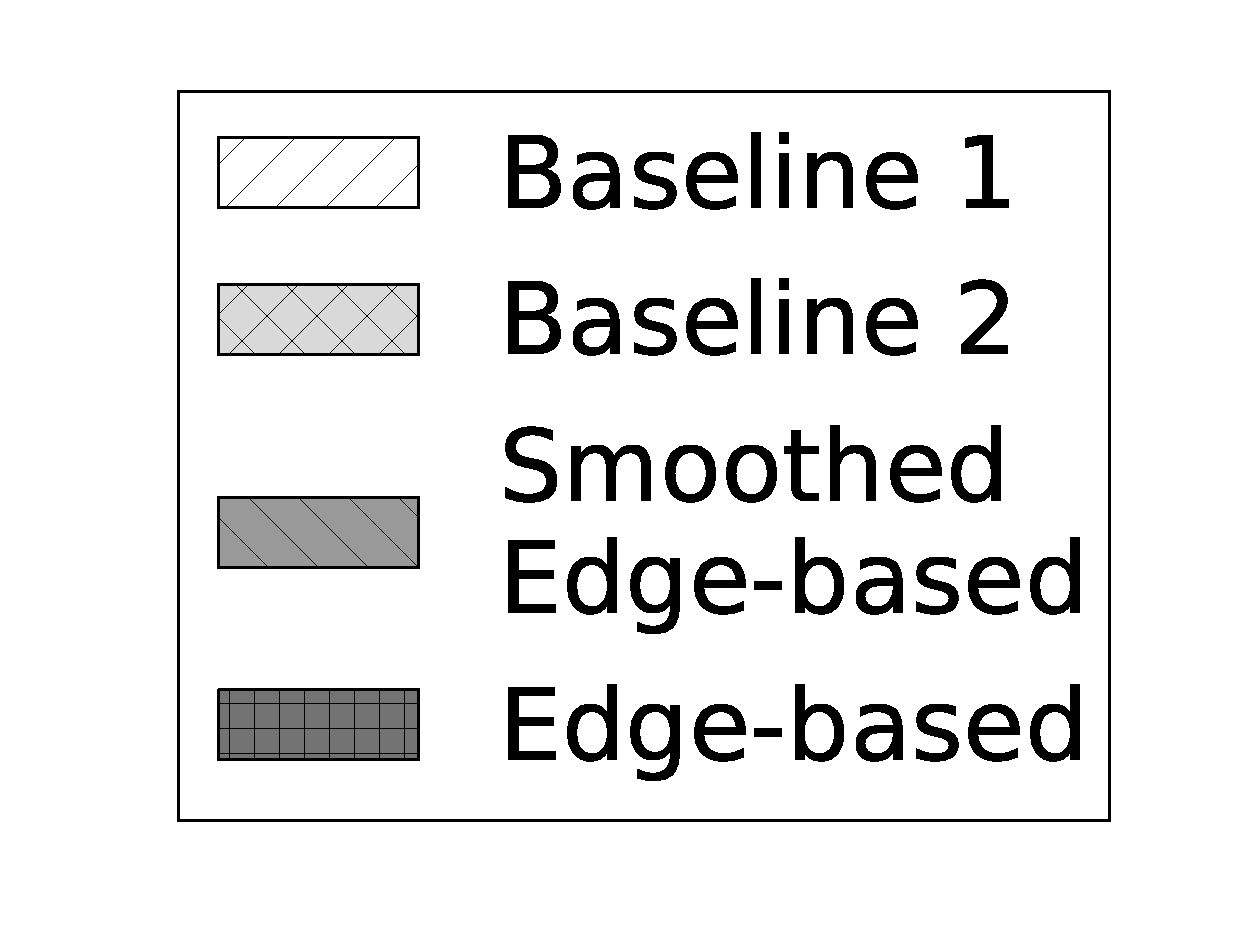
\includegraphics[width=1.6in]{legend} %3.3in is max!
		\caption{Legend}
		\label{fig:legend_train}
	\end{subfigure}
	\caption{Training Set: 5 Fold Cross Validation}
	\label{fig:5_fold_train}
\end{figure}

\begin{figure}[htb]
	\centering
	\begin{subfigure}{1.6in}
		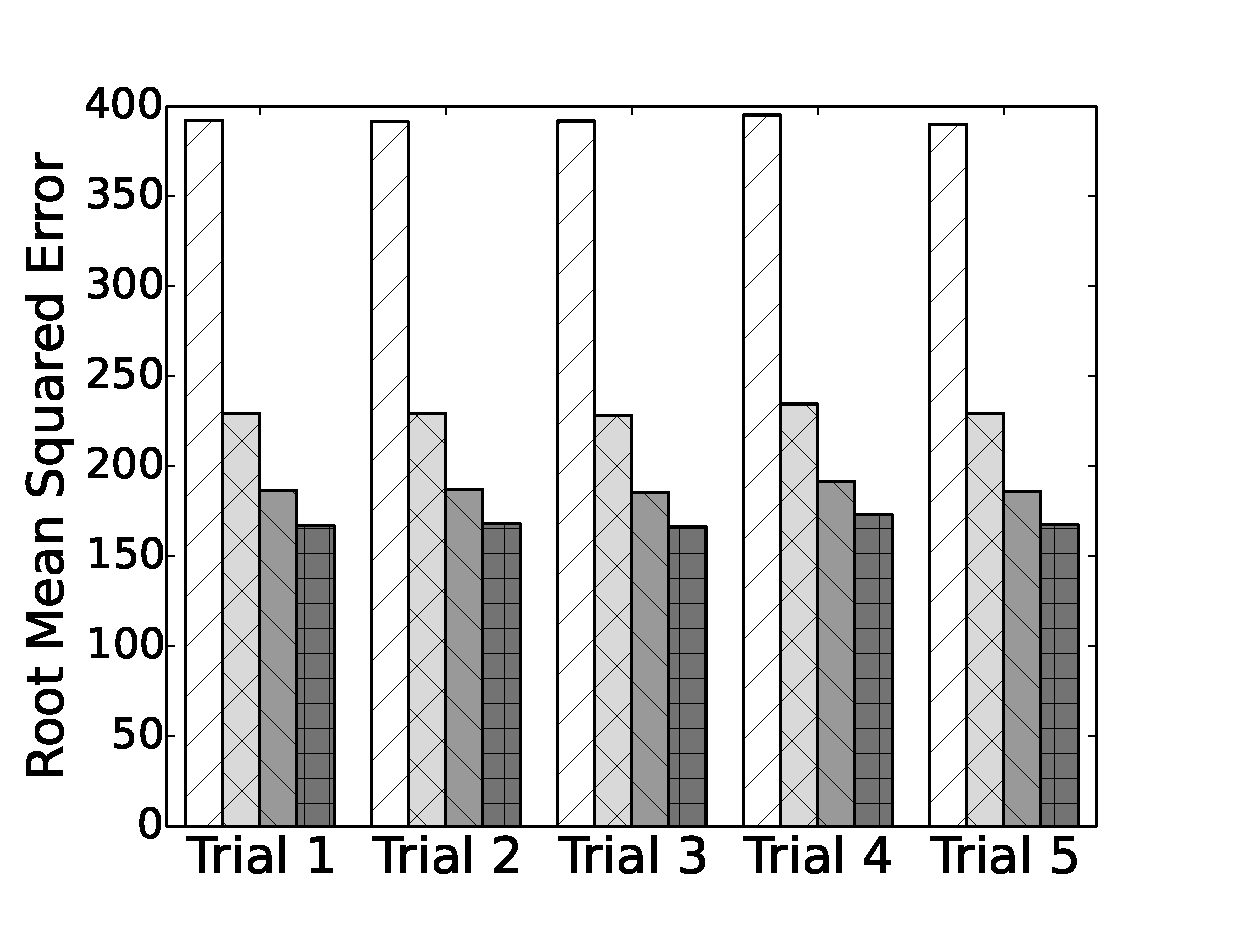
\includegraphics[width=1.6in]{20111208_test} %3.3in is max!
		\caption{Dec 8th 2011}
		\label{fig:20111208_test}
	\end{subfigure}
	\begin{subfigure}{1.6in}
		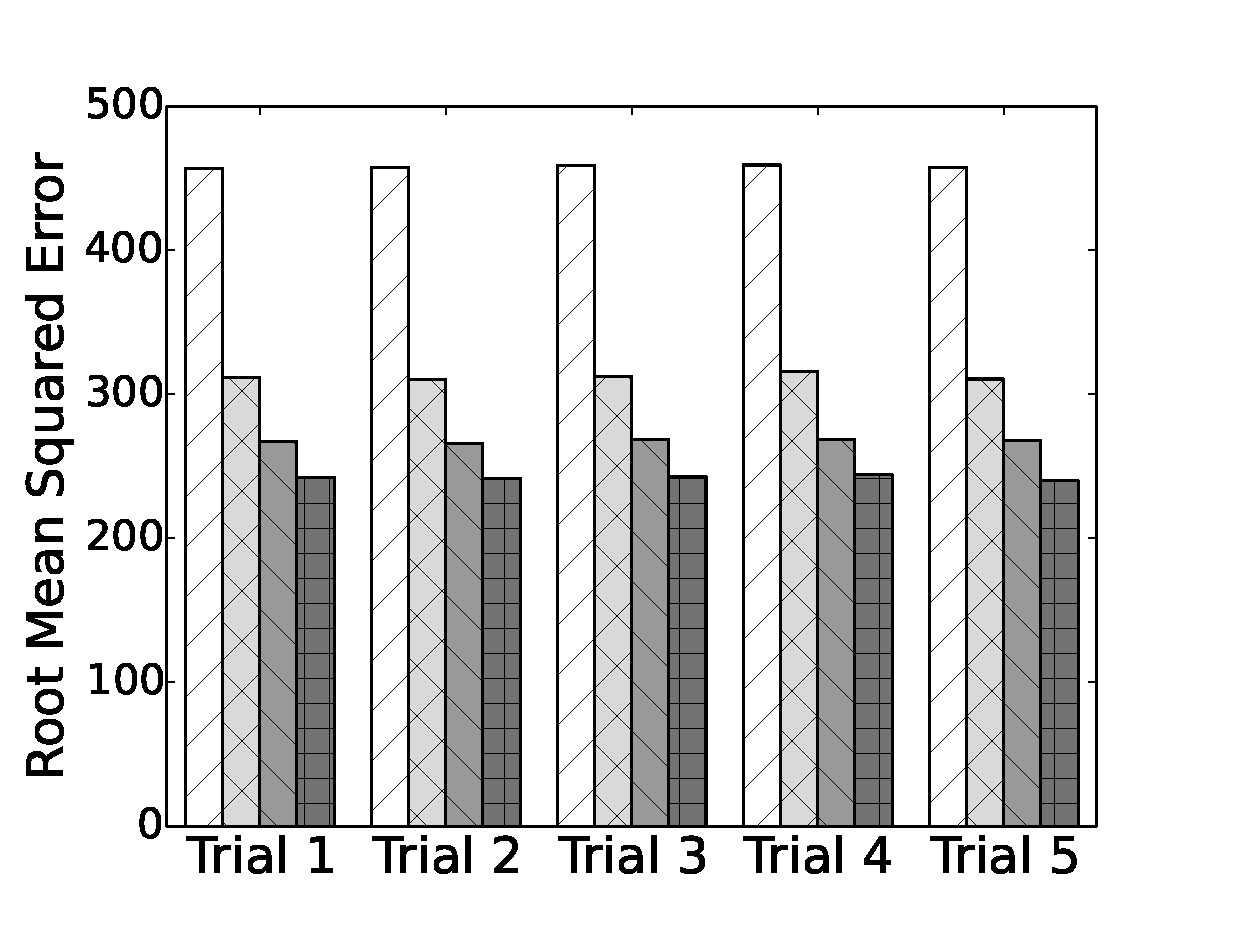
\includegraphics[width=1.6in]{20111215_test} %3.3in is max!
		\caption{Dec 15th 2011}
		\label{fig:20111215_test}
	\end{subfigure}
	\begin{subfigure}{1.6in}
		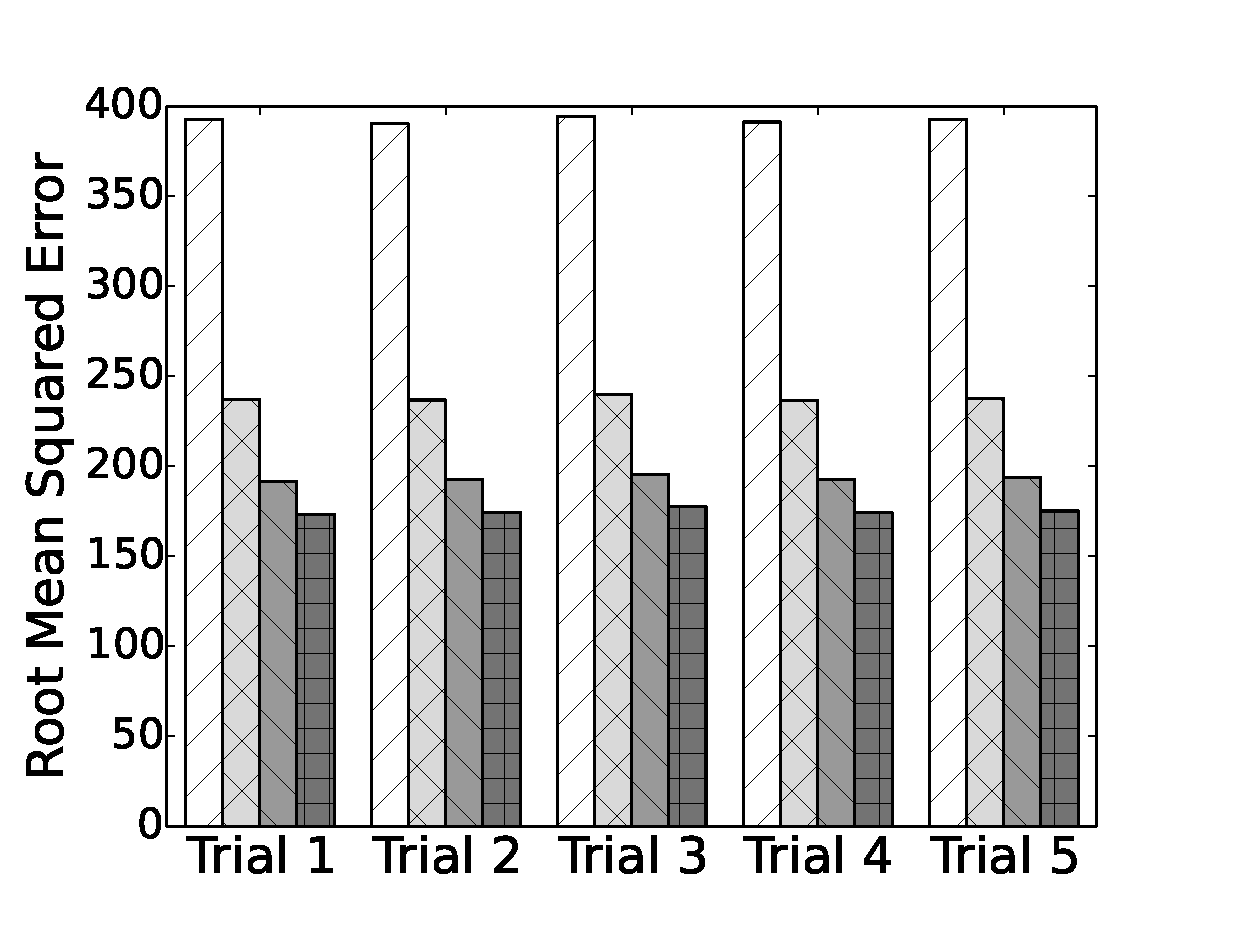
\includegraphics[width=1.6in]{20111222_test} %3.3in is max!
		\caption{Dec 22nd 2011}
		\label{fig:20111222_test}
	\end{subfigure}
	\begin{subfigure}{1.6in}
		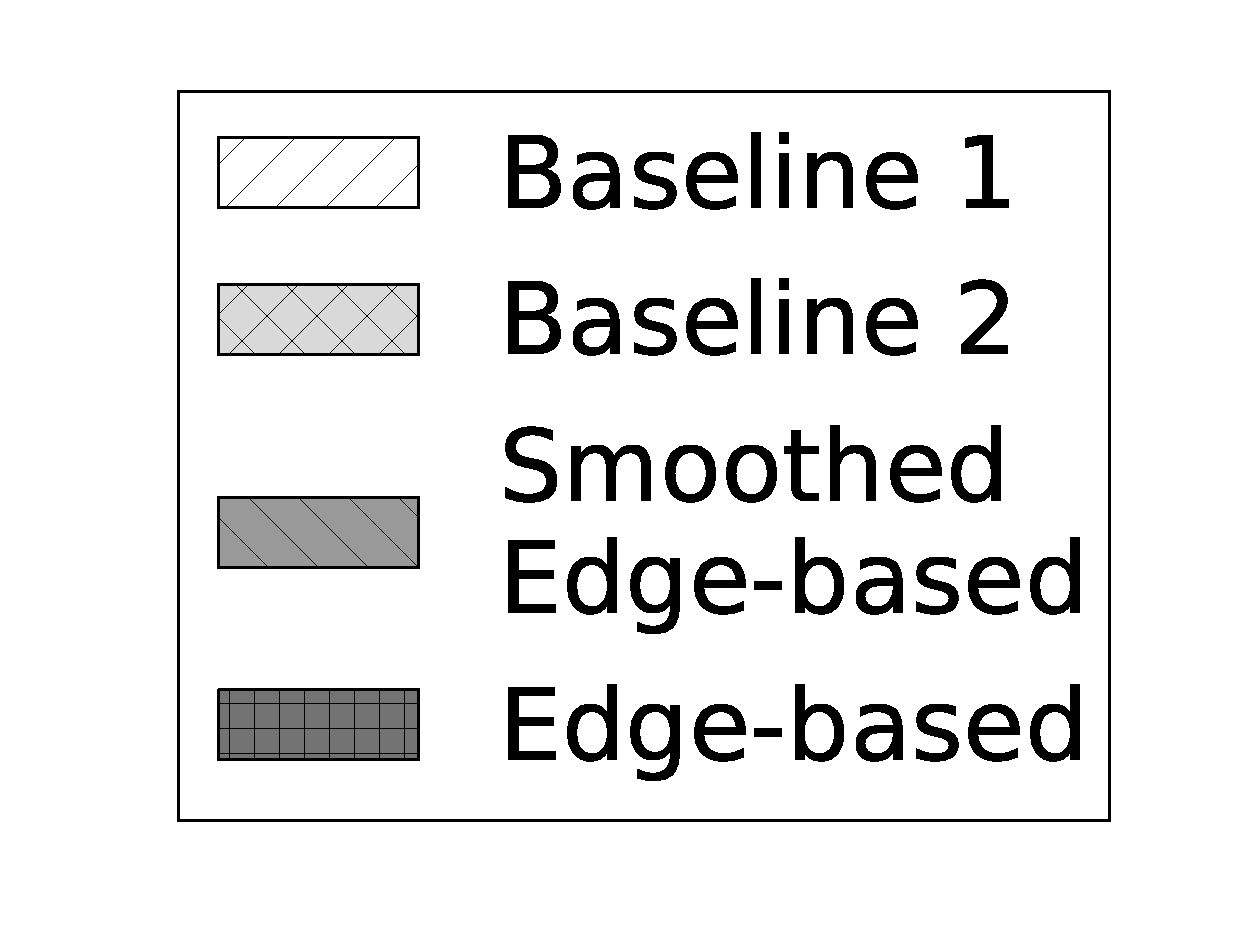
\includegraphics[width=1.6in]{legend} %3.3in is max!
		\caption{Legend}
		\label{fig:legend_test}
	\end{subfigure}
	\caption{Testing Set: 5 Fold Cross Validation}
	\label{fig:5_fold_test}
\end{figure}

\subsection{Case Studies on Anomalies}

\section{Conclusion}

\bibliographystyle{abbrv}
\bibliography{references}

\end{document}